\documentclass{article}

\usepackage{import}
\subimport{../preamble/}{lab_preamble.tex}

%
% Ideas:
% - make one of the resistors in the voltage divider a potentiometer and let the students twiddle it to see how the output voltage changes
% - use this to then introduce a three terminal potentiometer as a voltage divider itself
%




\title{Lab 1: Voltage, Current, Resistance, and Power}


\begin{document}
\maketitle

\section{Overview}
Electrical circuit design depends first and foremost on understanding the basic quantities used for describing electricity: voltage, current, and power. In the simplest circuits these are related by Ohm's law. After defining and understanding these quantities, we will begin a discussion of network analysis and look at a few examples.

\subsection{Voltage}
\emph{Voltage} (measured in volts, V) is electrical potential difference between two points in a circuit. You measure a voltage by connecting the two terminals of a \emph{voltmeter} to the two points in your circuit. You must measure the voltage while your circuit is operating. If you have a good voltmeter, your measured voltage will be the same as the voltage was before you connected the voltmeter. A voltage decrease in the direction of current flow represents energy flowing out of the circuit (usually into heat). Voltage sources, such as batteries and power supplies, produce voltage increases along the direction of current
flow.

\subsection{Current}
\emph{Current} (measured in amperes or amps, A, which is equivalent to Coulombs/second) is measured at a single point in a circuit. It is the rate at which charge flows along the circuit. To measure a current with a \emph{current meter (or ammeter)} you must break the circuit at that point and connect each end to one of the terminals of the ammeter. Current can only flow in complete circuits. That's why a switch stops an electrical circuit: it breaks the circuit and interrupts the current flow.

\subsection{\boldmath$IV$ Characteristic}
We can completely characterize any element that has two terminals by its $IV$ characteristic (i.e. how much current flows through it when a given voltage is put across it). The $IV$ characteristic is given by the functions $I(V)$ or $V(I)$ and is frequently defined graphically.  

\subsection{Ground}
\emph{Ground} is the name given to the V = 0 reference point. This makes it easier to refer to voltages, since you can generally assume that the second point is ground if it is not explicitly stated. We will also use it to represent the implied completion of a circuit, even when we do not explicitly show a wire connection between different places in a circuit, since all ground connections are connected together.

\subsection{Resistance}
A \emph{resistor} is a two-terminal device that converts a voltage into a current or converts a current into a voltage. The current through a resistor is always related to the voltage drop across the resistor by Ohm's Law
\begin{equation}
V = IR
\end{equation}
where $R$ is the resistance (measured in Ohms, $\Omega$) This also means that a resistor generates heat when a current flows given by:
\begin{equation}
 P = IV = I^2 R = \frac{V^2}{R}.
\end{equation}
Each of these expressions give the same answer but one or the other will be easier to use, depending on what you know about the circuit ($I$ or $V$, or both). It may seem silly to have a device that just turns electrical energy into heat, but resistors actually perform many important roles:
\begin{itemize}
\item They turn electrical energy into heat. This can be useful if you want to make an electrical heater, or (more likely) a light bulb. Light is just a form of heat given off by a very hot source. Sometimes you must dissipate power somewhere. For example, if you want to deliver 100\,mA current at 12\,V to part of your circuit, but your power supply gives you 15\,V, then the extra power
\begin{equation}
300\,mW = (100\,mA) (15\,V - 12\,V) 
\end{equation}
must go somewhere. You dissipate it in a resistor rather than by heating your sensitive transistors.
\item If you have a voltage source and you want a specific amount of current then a resistor does the job. It converts a voltage difference between two points into a current flowing through the resistor. Sometimes, you will add a resistor in series in a circuit to prevent the power supply from delivering too much current in case you short the output lines together. This is called a \emph{current limiting resistor}.
\item If you have a current flowing and you want to convert it into a voltage then a resistor is again the solution. This might seem a little more far-fetched, because you may not be familiar with constant current sources. When we begin studying transistors we will find that they will behave as \emph{current sources}. So we will use a resistor on the output to convert the current into a voltage.
\end{itemize}
When we consider capacitors, in week three, we will generalize resistance for AC circuits by allowing for phase shifts. We will call this generalization to the complex plane \emph{impedance}. For this week we will assume resistance and impedance to mean the same thing.

\section{Network Analysis}
If you connect one power supply and lots of resistors together in a complicated network, then currents will flow through all the various elements so as to insure that charge is conserved, energy is conserved, and Ohm's Law is satisfied. Simultaneously satisfying all these conditions will give you exactly one solution. We will start with two resistors and then proceed to more complicated systems. Specifically, two resistors in series will draw the same current as an equivalent resistor with resistance. This is stated mathematically as:
\begin{equation}
R_S = R_1 + R_2
\end{equation}
Alternatively, two resistors in parallel will draw current equivalent a resistor with resistance
\begin{equation}
\frac{1}{R_\parallel} = \frac{1}{R_1} + \frac{1}{R_2} \quad \hbox{or} \quad R_\parallel = \frac{R_1 R_2}{R_1 + R_2}
\end{equation}
Note that the resistance of 2 resistors in parallel is always less than the smaller, but not less than half of that smaller resistance. If the two resistors differ by a large factor, then you can ignore the larger resistor. For example, a 1\,k\Ohm in parallel with 1\,M\Ohm is within 999\,\Ohm or very close to 1\,k\Ohm.

Standard resistors come in a few dozen difference ratings (more on this in lab). So in general one can get any particular value one wants. One can make up an equivalent resistor using a few resistors in series and parallel combinations to get a much larger range of options. In Design Exercise 1-1, we have you design a network to have a specific net resistance given a very limited set of resistances.

\subsection{Voltage Dividers}
\begin{figure}
\centering
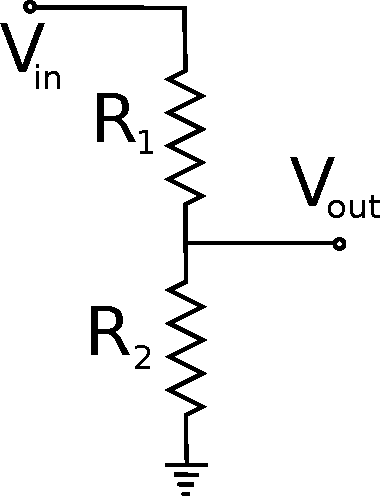
\includegraphics[height=0.2\textheight]{pics/unloaded_voltage_divider.pdf}
\caption{A voltage divider.}
\label{fig:unloaded_voltage_divider}
\end{figure}
By far the most useful thing you can do with two resistors is to make a \emph{voltage divider}, which is just two resistors in series. Voltage dividers are shown schematically in Figure~\ref{fig:unloaded_voltage_divider} in two slightly different but equivalent representations. It ``divides'' a total voltage into two parts with each part proportional to the resistance in that leg. So, if you know the starting voltage and the target voltage, then you can calculate the required ratio of the two resistors.
\begin{equation}
V_{out} = V_{in} \frac{R_2}{R_1 + R_2}
\end{equation}
In Design Exercise 1-2 you get to derive this relationship.

\subsection{Loaded Voltage Divider}
\begin{figure}
\centering
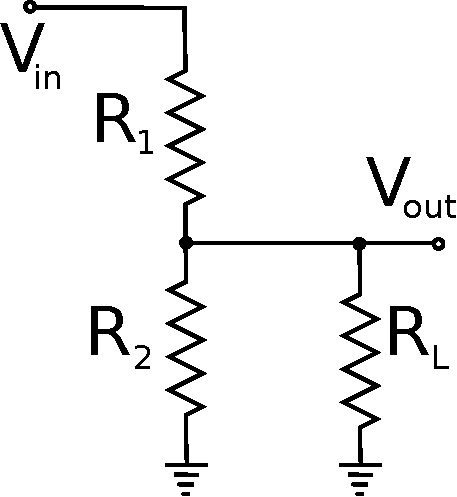
\includegraphics[height=0.2\textheight]{pics/loaded_voltage_divider.pdf}
\caption{A loaded voltage divider.}
\label{fig:loaded_voltage_divider}
\end{figure}
Of course, the way you will use $V_{out}$ from a voltage divider is to connect it to something, usually another resistor, as shown in Figure~\ref{fig:loaded_voltage_divider}. This then changes the equivalent resistance in the lower leg, and therefore changes the voltage across that leg!

In order to choose the actual resistor values, you have two competing concerns:
\begin{itemize}
\item low resistance makes the divider less sensitive to loading when you use the target voltage (i.e. ``stiffer''),
\item high resistance draws less current, and therefore uses less power.
\end{itemize}
We'll spend more time on this and formalize the considerations in the coming weeks. 

For now, let's just consider what happens to our voltage divider when we connect a load resistance ($R_L$) from its output to ground. In this case we can replace the $R_2$ from the expression for the unloaded divider with an equivalent resistance of $R_2$ and $R_L$ in parallel. This gives us a voltage across $R_L$ of:
\begin{eqnarray}
 V_{out,loaded} & = & V_{in} \frac{R_{2 \parallel L}}{R_1 + R_{2\parallel L}} \\
 & = & V_{out,unloaded} \frac{R_L}{R_L + R_{1||2}}
\end{eqnarray}
where $R_{2 \parallel L}$ is the equivalent resistance of $R_2$ and $R_L$ in parallel, $R_{1 \parallel 2}$ is the equivalent resistance of $R_1$ and $R_2$ in parallel, and $V_{out,unloaded}$ is the output voltage of the unloaded voltage divider. From the last expression it is clear that the loaded voltage is always less than the unloaded voltage. The smaller the load the larger the difference between loaded and unloaded, while large load resisters do not affect the output significantly. 

So, if you want to ensure that you do not affect the output of a device, you would like to have the input of your device to look like a large resistor and the output look (in this case $R_{1\parallel 2}$) look like a small resistance. Next week we'll show that this is a general conclusion and more formally define these concepts.


\pagebreak

\section{Lab 1: Design Exercises}

\begin{enumerate}
\item Design Exercise 1-1: Use only 10\,k\Ohm resistors to create a network with an equivalent resistance of 6.67\,k\Ohm. What is the minimum number of required resistors?
\item Design Exercise 1-2: Use network analysis and Ohm's Law to derive a formula for $V_{out}$­ for an unloaded voltage divider.
\item Design Exercise 1-3: Assuming that $R_1$, $R_2$ and $R_L$ are 10\,k\Ohm resistors and $V_{in}$ is 10\,V, compute $V_{out}$ for both a loaded voltage divider and an unloaded voltage divider­. How much does the output voltage change when it is loaded?
\end{enumerate}

\section{Lab 1: Voltage, Current, Resistance and Power}

\emph{Your notebooks must be complete, understandable, and address all activities, design exercises, observations, and questions noted in the laboratory's procedures. Remember to use your notebook as a laboratory journal and record your data, design calculations, notes and scratch work. Make sure to write a conclusion for each exercise and each week.} 

\begin{enumerate}
\item Measure the resistances of a few resistors with an ohmmeter and see how well they match their specified values. Are they within specifications, based on their tolerance bands?
\item Construct the resistor network you designed in Design Exercise 1-1. Check to see that the total resistance agrees with your calculation. Put 10\,V into your device and use an ammeter to see if it draws the expected current. How much power is being consumed, and how would one measure it?
\item Make a voltage divider from 1--100\,k\Ohm resistors and apply input voltages in the range of 2\,V--15\,V. Measure the input voltages and the current of this device. Be sure to sketch your experimental setup in your lab notebook! Plot your measurements with the voltage on the vertical axis and the current on the horizontal axis. The equivalent or input resistance of your voltage divider is the slope of the curve. Relate this to the resistors you used to construct the voltage divider.
\item Make your voltage divider from Design Exercise 1-3. Apply constant input voltage equal to 10\,V and measure the output voltage and output current for a variety of load resistances in the range from 100\,\Ohm to 100\,k\Ohm (use at least 10 different load resistors). Note how the output voltage changes and compare your results to your calculations. Do the results make sense?
\item Learn to start your oscilloscope and perform some basic tests. Feel free to consult the scope's manual to help you with the details as needed.
\begin{enumerate}
\item Select default configuration.
\item Connect a $10\times$ probe (look for a hardware switch on the probe) to channel 1, connect the ground to the scopes test ground, and connect the probe tip to the calibration test point on the front of the scope. You should see a square wave appear with a 1\,kHz frequency and 5\,V amplitude. 
\item Adjust the trim screw on the probe until the edges of the square wave are true (instead of rolling over or overshooting).
\item Verify the edges with a $1\times$ probe setting as well. 
\item Test the probe's calibration (i.e. do you get 1\,kHz and a 5\,V amplitude?). Record the result.
\item Zoom in and out on the signal and play with some of the measurements available to you on the scope (i.e. period, frequency, $V_{pp}$).
\end{enumerate}
\end{enumerate}

\end{document}
